\published{Geophysical Journal International, 222, 1824–1845, (2020)}

\title{Five-dimensional seismic data reconstruction using the optimally damped rank-reduction method}
\author{Yangkang Chen\footnotemark[1], Min Bai\footnotemark[1], Zhe Guan\footnotemark[2], Qingchen Zhang\footnotemark[1], Mi Zhang\footnotemark[3], and Hang Wang\footnotemark[1]}

\renewcommand{\thefootnote}{\fnsymbol{footnote}}

%\author{Yangkang Chen\footnotemark[1] et al.}

\ms{GJI-2020} %\ms{GJI-2018}

\address{
\footnotemark[1]
School of Earth Sciences\\
Zhejiang University\\
Hangzhou, Zhejiang Province, China, 310027\\
yangkang.chen@zju.edu.cn \\
%908352517@qq.com (hang)
\footnotemark[2]
Applied Physics Program\\
Rice University\\
Houston, TX, USA\\
%zg10@rice.edu
Zhe.Guan@rice.edu\\
\footnotemark[3]State Key Laboratory of Petroleum Resources and Prospecting \\
China University of Petroleum \\
Fuxue Road 18th\\
Beijing, China, 102200 \\
cupmi@sina.com \\
}

\lefthead{Chen et al., 2019}
\righthead{ORR}

\begin{abstract}
\old{We continue our previous work on simultaneous denoising and reconstruction of five-dimensional seismic data and propose a new algorithm, which is called optimal rank reduction method.} \old{The traditional rank reduction method is difficult to separate noise from signal by a typical truncated singular value decomposition (TSVD) strategy due to the mixture of the signal and the noise subspaces after the decomposition.} \new{It is difficult to separate additive random noise from spatially coherent signal using a rank-reduction method that is based on the truncated singular value decomposition (TSVD) operation. This problem is due to the mixture of the signal and the noise subspaces after the TSVD operation.} This drawback can be partially conquered \old{via}\new{using} a damped rank reduction method, where the singular values corresponding to effective signals are adjusted via a carefully designed damping operator. The damping operator works most powerfully in the case of a small rank and a small damping factor. However, for complicated seismic data, \new{e.g., multi-channel reflection seismic data containing highly curved events}, the rank should be large enough to preserve the details in the data, which makes the damped rank reduction method less effective. In this paper, we develop an optimal \old{weighting}\new{damping} strategy for adjusting the singular values \new{when a large rank parameter is selected} so that the estimated signal can best approximate the exact signal. \old{The optimal weighting strategy is inspired by the random matrix theory and can compute the optimal weighting coefficients directly from the observed data.}\new{We first weight the singular values using optimally calculated weights. The weights are theoretically derived by solving an optimization problem that minimizes the Frobenius-norm difference between the approximated signal components and the exact signal components. The damping operator is then derived based on the initial weighting operator to further reduce the residual noise after the optimal weighting. The resulted optimally damped rank reduction method is nearly an adaptive method, i.e., insensitive to the rank parameter.} We demonstrate the performance of the \old{optimal rank reduction method}\new{proposed method} on a group of synthetic and real five-dimensional seismic data.  \\
\textbf{Keywords}\\
Seismic noise, image processing, time-series analysis
\end{abstract}
%\section{Keywords}
%key1,key2,key3

\section{Introduction}
With the increasing demand for exploration accuracy, wide azimuth seismic (WAZ) exploration technology has received more and more attention and development. The seismic data obtained by WAZ acquisition contains rich wavefield information with high illumination \cite[]{yangkang20142,shuwei2016vscan,shaohuan2017gji,kim2017efficient,lu2017coal,tian2017characteristics,fly2017jse,kirchdepth2017jse,qushan2017eage,chenwei2018,qingchen2018gji,qingchen2018tgrs,yufeng2018geo}. However, due to the influence of surface environments, the shot, receiver, azimuth and offset of the original data tend to be unevenly distributed, which is adverse to the subsequent processing and interpretation such as migration, pre-stack attribute analysis, reservoir prediction and fluid identification. Seismic data interpolation is such a processing step to regularize the irregularly sampled seismic traces onto regular grids \cite[]{fomel2003,yangkang2016irr5d,shaohuan2016seg,yatong2018dbi,zhangdong2016seg,yangkang2016fwieage,yangkang2016fwi,zhangdong2016cseg,zhangdong2016eage}. In the past decades, a number of methods have been developed to reconstruct the missing seismic traces on regular grids. One widely used seismic reconstruction strategy is to transform the noisy seismic data into different domains in order to concisely represent the signal with a few number of selected components that capture the useful information and recover the missing components. These include the methods based on the Fourier transform \cite[]{yatong2017pocs,baimin2018jse2}, Radon transform \cite[]{beylkin1987discrete}, seislet transform \cite[]{shuwei20153,shuwei2015seg1,shuwei2015seg2,liuwei2016dealiase,zhiguang2017fwi,yatong2018seis,yatong2018jse,yangkang2018eseis,baimin2019jse1}, curvelet transform \cite[]{jianwei20093,candes20061,shaohuan2015,shaohuan2016seg2}, dreamlet transform \cite[]{benfengpocs}, wavelet transform \cite[]{rioul1991wavelets,gilles2013,xieqian2015eage,liuwei2016,mostafa2016bssa}, dictionary-learning based adaptive transform \cite[]{yangkang2016dsd,amir2017ieee,amir2017sp,amir2017geo,wujuan2018jge2,wujuan2018cg1,shaohuan2019ieee,shaohuan2019dl}. Another type of methods utilize the predictable property of seismic data. In the prediction-based approaches, a prediction error filter is designed such that the predicted data and the existing data have the minimum misfit by solving a least-squares linear inverse problem \cite[]{spitz1991,fomel2002pwd,yangkang2016irr5d}.  Considering the aliasing issue in reconstructing regularly sampled seismic data, a prediction error filter is first estimated from the aliasing-free low-frequency components and then applied to aliased high-frequency components \cite[]{mostafa2007}. The wave equation based methods can also be used to reconstruct highly incomplete seismic data. These methods connect the seismic record and the subsurface elastic properties via the elastic wave equation. However, these methods depend on a prior information about the subsurface elastic properties and are strictly not data-driven methods. In addition, these methods suffer from losing computational efficiency when applied in the interpolation methods \cite[]{ronen,canning1996,fomel2003}. A review of the latest methods on reconstructing low-dimensional seismic data is given in \cite{yangkang2019sg}.

However, the amplitude and phase variations of the WAZ seismic data are often not accurately recovered by conventional three-dimensional data reconstruction. More accurate reconstruction results can be obtained by simultaneously interpolating in five dimensions of inline, crossline, time, azimuth and offset because sampling along any particular subset of all dimensions is often less than ideal. The pre-stack seismic gathers processed by the five-dimensional (5D) interpolation have higher quality, which can not only improve the imaging accuracy, but also improve the capabilities of fracture prediction and fluid identification. Therefore, a large number of 5D seismic data reconstruction methods and techniques have emerged in the past decade.

The minimum weighted norm interpolation (MWNI) is a constrained inversion algorithm that was successfully applied to 5D seismic data interpolation \citep{Liubin2004, Trad2007, Trad2009}. \cite{Trad2007} employed this algorithm to regularize the data in the inline-crossline-azimuth-offset frequency domain and obtained pre-stack interpolated results for the migration input. This work proved that the results after 5D interpolation help to improve the fidelity of the migration, which laid the foundation for the subsequent promotion of five-dimensional seismic data reconstruction. \cite{Downton2008} confirmed the validity of the MWNI for 5D interpolation and found that the 5D interpolation can preserve the amplitude and improve the signal-to-noise ratio. The MWNI did successfully interpolate sparse data and reduced migration artifacts \citep{Trad2009}, but it had difficulty to deal regularly missing data with spatial aliasing. Chiu (2012) proposed an anti-aliasing MWNI method to improve the deficiency of conventional MWNI in processing aliased data. 
In addition, some other multidimensional interpolation algorithms are also available for the five dimensions \citep{Chopra2013}. \cite{Jin2010} proposed a 5D interpolation method based on a damped least-norm Fourier inversion (DLNFI). Benefiting from the use of nonuniform discrete Fourier transform, DLNFI breaks the limitation in MWNI that the input data must be binned into the regular grid. 

Another alternative 5D interpolation method utilizes wavefront attributes such as wavefront curvatures and propagation angles. \cite{Xie2017} proposed a wavefront-attribute-based 5D interpolation (5D WABI) via a global optimization strategy instead of pragmatic search approach, which can take advantage of the wide, rich, or full azimuth acquisitions. Application on a synthetic seismic data have shown that the 5D WABI method is better at preserving diffractions than the damped rank-reduction method but at the expense of significantly lower computational efficiency.
In recent years, dictionary learning and machine learning are applied to the reconstruction of 5D simple data \citep{YuSiwei2015, Jia2017, Jia2018}. Data driven tight frame (DDTF) is a kind of dictionary-learning method, which can simultaneously denoise and interpolate 5D seismic data \citep{YuSiwei2015}. In DDTF, a sparsity-promoting algorithm is used to build the dictionary which can represent the observed data and estimate the complete data. \cite{Jia2017} combined the DDTF with a classic machine learning method named support vector regression (SVR) to optimize the learning, which obtained better performance than the Gauss SVR method. With the continuous improvement of intelligent methods, learning-based 5D data reconstruction will be a hot research topic in the future.


Rank-reduction based algorithms have great potentials for 5D seismic data interpolation. \old{The starting point is that the fully sampled noise-free seismic data can be characterized as a low-rank matrix or tensor and the rank of the matrix or tensor increases when the missing traces and noise occur.}
\new{The basic assumption of these methods is that the fully sampled noise-free seismic data can be characterized as a low-rank matrix or tensor and the rank of the matrix or tensor increases when there are missing traces or noise in the data \cite[]{yatong2018gji}. The missing traces denote the zero-value seismic traces when the seismic data is binned from irregular station positions to regular grids.} 
By solving a low-rank tensor completion problem via convex optimization, the missing traces can be accurately recovered with the information of all dimensions \citep{Kreimer2013}. In addition, this method has stronger denoising ability than the previous methods. From other perspectives of rank minimization, \cite{Ely2015} estimated the complete data tensor via tensor singular value decomposition (SVD) and parallel matrix factorization, respectively. Subsequently, \cite{GaoJianjun2017} further developed a new and fast low-rank tensor completion method based on parallel square matrix factorization and advocated that reshaping the complete data tensor into almost square or square matrices can improve the reconstruction quality. However, when the signal-to-noise ratio of the observed seismic data is very low, \old{conventional}\new{the Cadzow} rank-reduction method\old{s} via truncated singular value decomposition (TSVD) do\new{es} not achieve \old{perfect}\new{reasonable} reconstruction result\old{, which is still filled with a large amount of residual noise}\new{, i.e., the result may still contains a large amount of residual noise}. \cite{yangkang2016irr5d} proposed a damped rank-reduction method to further suppress the residual noise by introducing a damping operator to the block Hankel matrix after TSVD. In the 5D reconstruction of field seismic data, the damped rank-reduction method achieved better performance than the \old{traditional }Cadzow rank-reduction method \citep{Trickett2009, mssa}. \new{Throughout the paper, the Cadzow rank-reduction method is referred to as the traditional rank-reduction method.} 

The basic assumption of the rank-reduction methods is that the Hankel matrix formulated from the useful seismic signal is of low rank and its rank is equal to the number of linear/planar events (or dipping components) in the seismic data \cite[]{mssa,weilin2016,amir2017grsl,yangkang2017lsrtm,yatong2018inter,wujuan2018jge1,wujuan2018jse1,wujuan2018jge3,baimin2018jse1,baimin2018cg,baimin2019jag,wujuan2019jse1}. However, in general the real seismic data is composed of nonlinear events, which are more complicated than the linear events. A common strategy for addressing this issue is to implement the algorithm in local patches since the events can be approximately viewed as linear in small patches \cite[]{zhangdong2017}. However, this strategy poses another difficulty of choosing an appropriate rank for each local processing window.  A practical implementation of the rank-reduction method may require the predefined rank to be relatively large in order to avoid the damage of useful signal due to inappropriate assumption of the structural complexity. This conservative selection of rank would make the resulted data contain a significant amount of residual noise. \old{In this paper, we develop an adaptive singular value weighting method by solving an optimization problem, by which we can suppress the strong residual noise even when using a large rank.}\new{In this paper, we develop a relatively adaptive rank-reduction method, by which we can suppress the strong residual noise even when using a large rank. We first calculate a set of optimal weighting coefficients to weight the singular values as a first step by solving an optimization problem that minimizes the Frobenius-norm difference between the approximated signal components and the exact signal components.} The rank-reduction method based on the optimal weighting strategy can be further improved when connected with the damped rank-reduction method. The resulted method is named as the \old{optimal}\new{optimally damped} rank-reduction method, and can \old{hopefully}\new{potentially} provide the \old{optimal}\new{best} solution to the rank-reduction based high-dimensional seismic reconstruction problem in an adaptive way. We will use comprehensive numerical tests and detailed analysis to demonstrate the superiority of the presented algorithm based on several synthetic examples and a real seismic data.


\section{Theory}
\subsection{Construction of the block Hankel matrix for 5-D seismic data}
Let $D(t,hx,hy,x,y)$ denote the 5-D seismic data in the time domain, and $D(f,hx,hy,x,y)$ be the data in the frequency domain. For notation convenience, we omit $f$ in the following context and use $D_{k1,k2,k3,k4}$ to denote $D(f,hx,hy,x,y)$. The \new{traditional} rank-reduction based methods require the construction of a level-four block Hankel matrix for 5-D seismic data to meet the low-rank assumption. \new{A level-four block Hankel matrix means that we treat a series of level-three block Hankel matrix as elements and arrange them into a Hankel matrix. In a similar way, a level-three block Hankel matrix is constructed from a series of level-two block Hankel matrices while a level-two block Hankel matrix is formed from several standard Hankel matrices. } 

The level-four block Hankel matrix has the following explicit expression:
\begin{equation}
\label{eq:levelfour}
\mathbf{H}^{(4)}=\left(\begin{array}{cccc}
\mathbf{H}_{1}^{(3)} & \mathbf{H}_{2}^{(3)} & \cdots & \mathbf{H}_{X_4-Y_4+1}^{(3)} \\
\mathbf{H}_{2}^{(3)} & \mathbf{H}_{3}^{(3)}  &\cdots & \mathbf{H}_{X_4-Y_4+2}^{(3)} \\
\vdots & \vdots &\ddots &\vdots \\
\mathbf{H}_{Y_4}^{(3)}&\mathbf{H}_{Y_4+1}^{(3)} &\cdots& \mathbf{H}_{X_4}^{(3)}
\end{array}
\right),
\end{equation}
where 
\begin{equation}
\label{eq:levelthree}
\mathbf{H}_{k4}^{(3)}=\left(\begin{array}{cccc}
\mathbf{H}_{1,k4}^{(2)} & \mathbf{H}_{2,k4}^{(2)} & \cdots &\mathbf{H}_{X_3-Y_3+1,k4}^{(2)} \\
\mathbf{H}_{2,k4}^{(2)} & \mathbf{H}_{3,k4}^{(2)}  &\cdots &\mathbf{H}_{X_3-Y_3+2,k4}^{(2)} \\
\vdots & \vdots &\ddots &\vdots \\
\mathbf{H}_{Y_3,k4}^{(2)}&\mathbf{H}_{Y_3+1,k4}^{(2)} &\cdots&\mathbf{H}_{X_3,k4}^{(2)}
\end{array}
\right),
\end{equation}
and 
\begin{equation}
\label{eq:leveltwo}
\mathbf{H}_{k3,k4}^{(2)}=\left(\begin{array}{cccc}
\mathbf{H}_{1,k3,k4}^{(1)} & \mathbf{H}_{2,k3,k4}^{(1)} & \cdots &\mathbf{H}_{X_2-Y_2+1,k3,k4}^{(1)} \\
\mathbf{H}_{2,k3,k4}^{(1)} & \mathbf{H}_{3,k3,k4}^{(1)}  &\cdots &\mathbf{H}_{X_2-Y_2+2,k3,k4}^{(1)} \\
\vdots & \vdots &\ddots &\vdots \\
\mathbf{H}_{Y_2,k3,k4}^{(1)}&\mathbf{H}_{Y_2+1,k3,k4}^{(1)} &\cdots&\mathbf{H}_{X_2,k3,k4}^{(1)}
\end{array}
\right),
\end{equation}
and

\begin{equation}
\label{eq:levelone}
\mathbf{H}_{k2,k3,k4}^{(1)}=\left(\begin{array}{cccc}
D_{1,k2,k3,k4} & D_{2,k2,k3,k4} & \cdots &D_{X_1-Y_1+1,k2,k3,k4} \\
D_{2,k2,k3,k4} & D_{3,k2,k3,k4}  &\cdots &D_{X_1-Y_1+2,k2,k3,k4} \\
\vdots & \vdots &\ddots &\vdots \\
D_{Y_1,k2,k3,k4}&D_{Y_1+1,k2,k3,k4} &\cdots&D_{X_1,k2,k3,k4}
\end{array}
\right).
\end{equation}

In order to make all target matrices (from equation \ref{eq:levelfour} to \ref{eq:levelone}) close to square matrices, parameters $Y_i$ are defined as $\lfloor \frac{X_i}{2} \rfloor +1$, $i=1,2,3,4$, where $X_i$ denotes the size of the $i$th dimension. Here, $\lfloor\cdot\rfloor$ denotes the integer part of an input argument.

The process of transforming a four-dimensional hypercube $D_{k1,k2,k3,k4}$ to the block Hankel matrix $\mathbf{H}^{(4)}$ is referred to as the Hankelization process. We can briefly denote this process as: 
\begin{equation}
\label{eq:hankel}
\mathbf{H}^{(4)}=\mathcal{H}D_{k1,k2,k3,k4}.
\end{equation}

Another important step in the rank-reduction based method is the rank reduction process, which can be denoted as $\mathcal{F}$. 

Reconstructing the missing data aims at solving \old{this problem}\new{the following equation}:
\begin{equation}
\label{eq:inv}
\mathcal{S} \circ \mathbf{M} = \mathbf{M}_{0},
\end{equation}
where $\mathcal{S}$ is a sampling matrix, $\mathbf{M}=\mathbf{H}^{(4)}$, and $\mathbf{M}_{0}$ denotes the block Hankel
matrix with missing entries. $\circ$ denotes element-wise product.

Equation \ref{eq:inv} is seriously ill-posed and the low-rank assumption is applied to constrain the model,
\begin{equation}
\label{eq:inv2}
\begin{split}
\min_{\mathbf{M}} &\parallel \mathcal{S} \circ \mathbf{M}-\mathbf{M}_{0}\parallel_F, \\
\text{s.t.}&\quad \text{rank}(\mathbf{M})=N.
\end{split}
\end{equation}
\new{$\parallel \cdot \parallel_F$ denotes the Frobenius norm of an input matrix. The constraint in equation \ref{eq:inv2} means that we constrain the rank of the block Hankel matrix to be $N$.}


The problem expressed in equation \ref{eq:inv2} can be solved via the following iterative solver:
\begin{equation}
\label{eq:iter}
\mathbf{M}_n=a_n \mathbf{M}_{0} + (1-a_n\mathcal{S})\circ \mathcal{F}\mathbf{M}_{n-1},
\end{equation}
$a_n$ is an iteration-dependent scalar that linearly decreases from $a_1=1$ to $a_{n_{max}}=0$. $a_n$ is used to alleviate the influence of random noise existing in the observed data. 

\subsection{Optimal weighting for rank reduction}
The observed data $\mathbf{M}$ can be expressed as:
\begin{equation}
\label{eq:msn}
\mathbf{M}=\mathbf{S}+\mathbf{N},
\end{equation}
where $\mathbf{S}$ and $\mathbf{N}$ denote the signal and noise components. \new{It is worth noting that for the derivation convenience, we assume the noise component $\mathbf{N}$ to be white. Although not exactly correct for seismic data, the denoising model also works for seismic data with band-limited noise.} In the following analysis, we assume $\mathbf{M}$ and $\mathbf{N}$ have full rank and $\mathbf{S}$ has deficient rank. $\mathbf{M}$, $\mathbf{S}$ and $\mathbf{N}$ are all of size $I\times J$.

The singular value decomposition (SVD) of $\mathbf{S}$ can be represented as:
\begin{equation}
\label{eq:svds_a}
\mathbf{S} = [\mathbf{U}_1^{S}\quad \mathbf{U}_2^{S}]\left[\begin{array}{cc}
\boldsymbol{\Sigma}_1^{S} & \mathbf{0}\\
\mathbf{0} & \boldsymbol{\Sigma}_2^{S}
\end{array}
\right]\left[\begin{array}{c}
(\mathbf{V}_1^{S})^H\\
(\mathbf{V}_2^{S})^H
\end{array}
\right].
\end{equation}
Because of the deficient rank, the matrix $\mathbf{S}$ can be written as:
\begin{equation}
\label{eq:S_a}
\mathbf{S}=\mathbf{U}_1^S\boldsymbol{\Sigma}_1^S(\mathbf{V}_1^S)^H.
\end{equation}

The singular value decomposition (SVD) of $\mathbf{M}$ can be represented as:
\begin{equation}
\label{eq:svdm_a}
\mathbf{M} = [\mathbf{U}_1^{M}\quad \mathbf{U}_2^{M}]\left[\begin{array}{cc}
\boldsymbol{\Sigma}_1^{M} & \mathbf{0}\\
\mathbf{0} & \boldsymbol{\Sigma}_2^{M}
\end{array}
\right]\left[\begin{array}{c}
(\mathbf{V}_1^{M})^H\\
(\mathbf{V}_2^{M})^H
\end{array}
\right].
\end{equation}
The rank-reduction method by TSVD refers to 
\begin{equation}
\label{eq:M_a}
\tilde{\mathbf{M}}=\mathbf{U}_1^M\boldsymbol{\Sigma}_1^M(\mathbf{V}_1^M)^H.
\end{equation}
Here, $\tilde{\mathbf{M}}$ is the estimated signal component via TSVD. We assume the \old{appealing rank}\new{rank} of $\mathbf{M}$ is $N$, and thus the size of $\mathbf{U}_1^M$ is $I\times N$. $\boldsymbol{\Sigma}_1^M$ is of size $N\times N$. $\mathbf{V}_1^M$ is of size $J\times N$.


However, the $\tilde{\mathbf{M}}$ is still a mixture of the signal and noise subspaces. Combining equations \ref{eq:msn}, \ref{eq:svds_a}, and \ref{eq:S_a}, it is easy to derive that \cite[]{yangkang2016irr5d}
\begin{equation}
\label{eq:msn2}
\tilde{\mathbf{M}}=\mathbf{S}+\mathbf{U}_1^S(\mathbf{U}_1^S)^H\mathbf{N},
\end{equation}
where we can see that the estimated signal component via TSVD is still corrupted by the noise component, which is the projection of the noise component to the signal component.

This problem can be partially alleviated by a singular value thresholding step:
\begin{equation}
\label{eq:M_a}
\tilde{\tilde{\mathbf{M}}}=\mathbf{U}_1^M\tilde{\boldsymbol{\Sigma}}_1^M(\mathbf{V}_1^M)^H,
\end{equation}
where $\tilde{\boldsymbol{\Sigma}}_1^M$ is the thresholded singular values such that:
\begin{equation}
\label{eq:thr}
\tilde{\boldsymbol{\Sigma}}_1^M = \mathbf{T}(\boldsymbol{\Sigma}_1^M,\tau).
\end{equation}
where $\mathbf{T}$ denotes a singular value thresholding operator and $\tau$ denotes the threshold. However, defining an optimal threshold is inconvenient and sometimes even difficult. It is because the noise component contributes differently to each singular value and a constant threshold is not plausible to deal with the inhomogeneous noise distribution. 

Thus, in this paper, we propose an adaptive weighting algorithm to optimally define the singular values in order to best reconstruct the signal component. We introduce a weighting operator $\mathbf{W}$ to adjust the $\boldsymbol{\Sigma}_1^M$ after applying SVD to the observed noisy signal. To calculate the optimal weighting operator is equivalent to solving the following optimization problem:
\begin{equation}
\label{eq:opt}
\hat{\mathbf{W}} = \arg \min_{\mathbf{W}} \parallel \mathbf{U}_1^S\boldsymbol{\Sigma}_1^S(\mathbf{V}_1^S)^H - \mathbf{U}_1^M\mathbf{W}\boldsymbol{\Sigma}_1^M(\mathbf{V}_1^M)^H \parallel_F.
\end{equation}
By an optimally weighted combination of estimated left and right singular vectors, the optimization problem \ref{eq:opt} can yield the optimally adjusted singular values to obtain the closest low-rank estimates of signal component. 

The optimal solution for the optimization problem was given in \cite{Benaych2012The} and \cite{optshrink2013}:
\begin{equation}
\label{eq:optW}
\hat{\mathbf{W}} = \text{diag}(\hat{w}_1,\hat{w}_2,\cdots,\hat{w}_N),
\end{equation}
where
\begin{equation}
\label{eq:optw}
\hat{w}_i=\left(-\frac{2}{\sigma_i^M}\frac{D(\sigma_i^M;\boldsymbol{\Sigma})}{D'(\sigma_i^M;\boldsymbol{\Sigma})}\right).
\end{equation}
$\sigma_i^M$ denotes the $i$th diagonal entry of $\boldsymbol{\Sigma}_1^M$ ($\boldsymbol{\Sigma}_1^M\in\mathbb{R}^{N\times N}$). $D$ denotes the D-transform:
\begin{equation}
\label{eq:D1}
\begin{split}
D(\sigma;\boldsymbol{\Sigma})&= \frac{1}{N} \text{Tr}\left(\sigma(\sigma^2\mathbf{I}-\boldsymbol{\Sigma}\boldsymbol{\Sigma}^H)^{-1}\right)\frac{1}{N} \text{Tr}\left(\sigma(\sigma^2\mathbf{I}-\boldsymbol{\Sigma}^H\boldsymbol{\Sigma})^{-1}\right)\\
&=\left[\frac{1}{N} \text{Tr}\left(\sigma(\sigma^2\mathbf{I}-\boldsymbol{\Sigma}^2)^{-1}\right)\right]^2
\end{split},
\end{equation}
where $D'$ is the derivative of $D$ with respect to $\sigma$, and $\text{Tr}(\cdot)$ is the trace of the input:
\begin{equation}
\label{eq:D2}
\begin{split}
D'(\sigma;\boldsymbol{\Sigma})&= 2\left[\frac{1}{N} \text{Tr}\left(\sigma(\sigma^2\mathbf{I}-\boldsymbol{\Sigma}^2)^{-1}\right)\right]\left[\frac{1}{N} \text{Tr}\left((\sigma^2\mathbf{I}-\boldsymbol{\Sigma}^2)^{-1}-2\sigma(\sigma^2\mathbf{I}-\boldsymbol{\Sigma}^2)^{-2}\sigma\right)\right] \\
&=\frac{2}{N^2}\left[ \text{Tr}\left(\sigma(\sigma^2\mathbf{I}-\boldsymbol{\Sigma}^2)^{-1}\right)\right]\left[ \text{Tr}\left((\sigma^2\mathbf{I}-\boldsymbol{\Sigma}^2)^{-1}-2\sigma^2(\sigma^2\mathbf{I}-\boldsymbol{\Sigma}^2)^{-2}\right)\right].
\end{split}
\end{equation}
Using the optimally estimated weighting operator expressed in equation \ref{eq:optW}, we can expressed the optimally estimated signal component as:
\begin{equation}
\label{eq:M_a}
\hat{\mathbf{M}}=\mathbf{U}_1^M\hat{\mathbf{W}}\boldsymbol{\Sigma}_1^M(\mathbf{V}_1^M)^H.
\end{equation}

\new{The optimal weighting strategy of the singular values is a substitute to directly truncating the singular values as used in the traditional rank-reduction method. An early investigation of the strategy to improve the rank-reduction performance in seismic data denoising and reconstruction is presented in \cite{aharchaou2017singular}. Besides, there are also a number of alternatives to these two approaches (weighting and truncating) such as  automatic rank determination \cite[]{gavish2014optimal,trickett2015preserving} and randomized approaches such as the randomized SVD and randomized QR factorizations \cite[]{jinkun2016}.}


\new{\subsection{Optimally damped rank-reduction method}}
\new{In this section, we will derive a damping operator for the optimally estimated signal components to further reduce the residual noise after rank reduction.}
Let 
\begin{equation}
\label{eq:svds_q}
\mathbf{Q} = [\mathbf{U}_1^{Q}\quad \mathbf{U}_2^{Q}]\left[\begin{array}{cc}
\boldsymbol{\Sigma}_1^{Q} & \mathbf{0}\\
\mathbf{0} & \boldsymbol{\Sigma}_2^{Q}
\end{array}
\right]\left[\begin{array}{c}
(\mathbf{V}_1^{Q})^H\\
(\mathbf{V}_2^{Q})^H
\end{array}
\right].
\end{equation} to be an SVD of matrix $\mathbf{Q}$,
and let
\begin{align}
\label{eq:svds_qu}
\mathbf{U}_1^{Q} = \mathbf{U}_1^{M},\\
\label{eq:svds_qs}
\boldsymbol{\Sigma}_1^{Q} = \hat{\mathbf{W}}\boldsymbol{\Sigma}_1^{M},\\
\label{eq:svds_qv}
\mathbf{V}_1^{Q} = \mathbf{V}_1^{M},
\end{align}
then equation \ref{eq:M_a} can be understood as a TSVD of the matrix $Q$:
\begin{equation}
\label{eq:tsvdq}
\tilde{\mathbf{Q}}=\mathbf{U}_1^{Q}\boldsymbol{\Sigma}_1^{Q}{\mathbf{V}_1^{Q}}^H.
\end{equation}
 Analogous to equation \ref{eq:msn2}, 
equation \ref{eq:M_a} can be re-formulated as 
\begin{equation}
\label{eq:M_a3}
\tilde{\mathbf{Q}}=\hat{\mathbf{M}}=\tilde{\mathbf{S}}+\mathbf{U}_1^{\tilde{\mathbf{S}}}{\mathbf{U}_1^{\tilde{\mathbf{S}}}}^H\tilde{\mathbf{N}},
\end{equation}

When the \old{appealing rank}\new{rank} is sufficiently large, we assume the estimated signal contains all signal components of the originally observed noisy data and contains less noise than the observed data. To further suppress the residual noise in the estimated signal, we re-analyze $\hat{\mathbf{M}}$ in detail. We can express the newly estimated signal as:
\begin{equation}
\label{eq:M_a2}
\tilde{\mathbf{Q}}=\hat{\mathbf{M}}=\mathbf{S}+\mathbf{U}_1^{S}{\mathbf{U}_1^{S}}^H\tilde{\mathbf{N}},
\end{equation}
where $\mathbf{U}_1^{S}{\mathbf{U}_1^{S}}^H\tilde{\mathbf{N}}$ denotes the residual noise component after the step using equation \ref{eq:M_a}.

Following \cite{yangkang2016irr5d} and \cite{weilin2016}, $\mathbf{S}$ can be approximated as:
\begin{align}
\label{eq:S3}
\mathbf{S} &= \mathbf{U}_1^{Q}\boldsymbol{\Sigma}_1^{Q}\mathbf{T}\left(\mathbf{V}_1^{Q}\right)^H,\\
\label{eq:T}
\mathbf{T} &= \mathbf{I}-\boldsymbol{\Gamma},
\end{align}
where $\mathbf{I}$ is a unit matrix and here we name $\mathbf{T}$ the damping operator. The damping relation $\boldsymbol{\Gamma}$ is expressed as:
\begin{equation}
\label{eq:Gamma}
\boldsymbol{\Gamma} \approx \hat{\delta}^N\left(\boldsymbol{\Sigma}_1^{Q}\right)^{-N},
\end{equation}
where $\hat{\delta}$ denotes the maximum element of $\boldsymbol{\Sigma}_2^{Q}$ and $N$ denotes the damping factor. 

Considering that $\mathbf{U}_1^{Q} = \mathbf{U}_1^{M}$, $\boldsymbol{\Sigma}_1^{Q}= \hat{\mathbf{W}}\boldsymbol{\Sigma}_1^{M}$, and $\mathbf{V}_1^{Q} = \mathbf{V}_1^{M}$,  equation \ref{eq:S3} can be expressed as:
\begin{align}
\label{eq:S33}
\mathbf{S} = \mathbf{U}_1^{M} \mathbf{T} \hat{\mathbf{W}}\boldsymbol{\Sigma}_1^{M} \left(\mathbf{V}_1^{M}\right)^H,
\end{align}
which is referred to as the \old{optimal rank reduction}\new{optimally damped rank reduction} method. The $\mathcal{F}$ can thus be chosen as the operation defined in equation \ref{eq:S33}, and through iterations we can reconstruct and denoise the 5D frequency-domain seismic data. 


\new{There are two main advantages of the optimally damped rank reduction method.  First, compared with the traditional and damped rank-reduction methods, the optimally damped rank reduction method is insensitive to the rank parameter, making it nearly an adaptive method for rank reduction based seismic denoising and reconstruction. This advantage is important because one of the most troublesome problems in processing complicated seismic data is the selection of the rank. A large rank tends to result in significant residual noise while a small rank tends to damage useful signals. This parameterization problem becomes more seriously when the rank reduction method is applied locally in windows. Because of the insensitivity to rank of the proposed method, one can choose a relatively large rank for all complicated datasets or local patches. Secondly, compared with the optimal weighting based rank reduction method, the proposed method can further suppress the noise components that reside mostly in the smaller singular values. The damping operator is data-driven and can adaptively separate signal and noise in the singular value spectrum further after the optimal weighting.  }

\new{In the rank-reduction methods, construction of the level-four Hankel matrix is very computationally expensive.  Recent advances in the rank reduction based methods show that the construction of the block Hankel matrix is not required. These methods exploit the structure of such matrices to avoid explicitly forming these matrices prior to factorization \cite[]{lu2015fast,cheng2016fast}. When factorizing data using only 1 or 2 spatial dimensions these approaches are not necessary, but moving to 3 or 4 spatial dimensions is not computationally feasible without considering matrix free approaches. In the current stage, we cannot move from the SVD-based method to SVD-free method because the damping operation has not been derived for the SVD-free case. Although it takes a large computational cost and is not very practically for the time being, it is still a promising algorithm. We will keep on investigating the acceleration of the current algorithm and make it computationally feasible in the future.}

\section{Examples}
We first apply the proposed optimal rank-reduction method to a 5D synthetic data with linear/planar events, as shown in Figure \ref{fig:figure1}. Figure \ref{fig:figure1}(a) shows the clean synthetic data in a common offset gather. The 3D common offset gather ($t-x-y$) has been arranged into a 2D matrix. Figure \ref{fig:figure1}(b) shows the noisy data with extremely strong band-limited random noise. The useful signals are almost buried in the strong noise. Figure \ref{fig:figure1}(c) shows the incomplete data, where 75\% traces have been randomly decimated. The reconstructed and denoised data using three different methods, i.e., the traditional rank-reduction method (RR), the damped rank-reduction method (DRR), and the \old{optimal}\new{optimally damped} rank-reduction method (ORR), are shown in Figure \ref{fig:figure2}. All three methods successfully recovered most of the signals.  It is clear that the RR method causes significant residual noise, the result from the DRR method is much cleaner than that from the RR method but still contains some residual noise. The proposed ORR method, however, obtains the cleanest result among the three results shown in Figure \ref{fig:figure2}. To evaluate the quality of the three reconstructed data, given the exact solution in Figure \ref{fig:figure1}(a), we calculate the local similarity map between each reconstructed data and the exact solution. The local similarity is a way to evaluate the similarity between two vectors/matrices/cubes in a local manner so that the evaluation can be revealed immediately from the calculated local similarity maps. The detailed introduction of mathematics behind the local similarity calculation can be found in \cite{yangkang2015ortho}. From the local similarity comparison, it is quite obvious that from the top panel (RR method) to the bottom panel (ORR method), the similarity becomes higher and higher, which indicates that the proposed method obtains the most accurate solution.

To examine the amplitude recovery quality, we select the 22nd traces from the clean data in Figure \ref{fig:figure1}(a) and from the three reconstructed data in Figure \ref{fig:figure2}, and draw them in Figure \ref{fig:figure4}. Figure \ref{fig:figure4}(a) shows the trace-by-trace comparison in the range of the whole trace and Figure \ref{fig:figure4}(b) shows the zoomed trade-by-trace comparison. The zooming part is highlighted by the red transparent rectangle shown in Figure \ref{fig:figure4}(a). From Figure \ref{fig:figure4} we can see that both RR and DRR methods (blue and red lines) cause strong fluctuations in the front part of the trace, while the proposed method obtains a result (the green line) that is the closest to the exact solution (the black line). The observation is even clearer in the zoomed comparison shown in Figure \ref{fig:figure4}(b). Figure \ref{fig:figure5} shows the comparison of reconstruction error. The reconstruction error is calculated as the difference between the exact solution (Figure \ref{fig:figure1}(a)) and each reconstructed data shown in Figure \ref{fig:figure2}. From Figure \ref{fig:figure5} we can observe that both RR and DRR cause significant error and the proposed ORR method causes negligible reconstruction error except for some observable signal energy. The reconstruction error of RR method is higher than the DRR method, mostly because of the stronger residual noise caused by the RR method. Since the reconstruction error for the proposed method is mostly negligible, the error caused by the leakage signal energy becomes more apparent. To compare the leakage signal energy among three methods, we calculate the extra noise section of the RR and DRR methods. The extra noise section refers to the extra noise compared with the reference noise section from the ORR method (Figure \ref{fig:figure5}(c)), thus is calculated as the difference between the error from either RR or DRR method and the error from the ORR method. The extra noise sections corresponding to the RR and DRR methods are shown in Figure \ref{fig:figure6}. It is obvious that by calculating the extra error sections, the leakage useful energy from RR/DRR method and ORR method counteract each other and the resulting sections are mostly random noise. This observation indicates that the energy of the leakage signal for the three methods are nearly the same. We conclude from this test that despite the same damage to useful signals, the proposed method causes the least residual noise and thus obtains the cleanest reconstruction result.

We also compare the level-four block Hankel matrices of different methods. Figures \ref{fig:H_clean} and \ref{fig:H_obs} shows the Hankel matrices for the clean and incomplete data for the frequency slice of 30Hz. Figures \ref{fig:H-z-clean} and \ref{fig:H-z-obs} show the zoomed Hankel matrices for the clean and incomplete data. The zooming areas are highlighted by the red rectangles shown in Figures \ref{fig:H_clean} and \ref{fig:H_obs}. Because of the missing traces, the Hankel matrix contains a number of blank areas. Figure \ref{fig:H_rr1,H_rr10,H_drr1,H_drr10,H_odrr1,H_odrr10} shows the Hankel matrices for different methods. The left column correspond to the Hankel matrices after 1 iteration. The right column correspond to the Hankel matrices after 10 iterations. We only conclude from Figure \ref{fig:H_rr1,H_rr10,H_drr1,H_drr10,H_odrr1,H_odrr10} that after 10 iterations all three methods obtain similar Hankel matrices as the exact solution shown in Figure \ref{fig:H_clean} but we cannot see the difference between different methods clearly. The differences between different methods can be clearly observed from the zoomed Hankel matrices, as shown in Figure \ref{fig:H-z-rr1,H-z-rr10,H-z-drr1,H-z-drr10,H-z-odrr1,H-z-odrr10}. It is clear that from the top to bottom in Figure \ref{fig:H-z-rr1,H-z-rr10,H-z-drr1,H-z-drr10,H-z-odrr1,H-z-odrr10}, the Hankel matrix becomes smoother and smoother and is closer to the exact solution shown in Figure \ref{fig:H-z-clean}. 

In addition to the local similarity mentioned above, we also use the signal-to-noise ratio (SNR) defined as follows to quantitatively measure the performance \cite[]{weilin2016,yangkang2017sgk,weilin2017gji}:
\begin{equation}
\label{eq:dsnr}
SNR=10\log_{10}\frac{\Arrowvert \mathbf{s} \Arrowvert_2^2}{\Arrowvert \mathbf{s} -\hat{\mathbf{s}}\Arrowvert_2^2}.
\end{equation}
where $\mathbf{s}$ denotes the vectorized clean data and $\hat{\mathbf{s}}$ denotes the vectorized reconstructed data. In this example, the SNRs of the observed data, the reconstructed results via the RR method, the DRR method, and ORR method are -4.59 dB, 5.51 dB, 9.54 dB, and 11.83 dB, respectively. In this test, we use $rank=10$, assuming that we do not have a prior information about the structural complexity of the data and thus needing to set a relatively high rank. We then test the performance when the rank is chosen smaller. The reconstructed data when $rank=5$ are shown in Figure \ref{fig:figure10}. Their corresponding error sections are shown in Figure \ref{fig:figure11}. From Figures \ref{fig:figure10} and \ref{fig:figure11}, we can reach almost the same conclusion as the last test. In this case, the SNRs of the reconstructed results via the RR method, the DRR method, and ORR method are 8.01 dB, 10.87 dB, and 11.97 dB, respectively. The detailed SNR comparison is shown in Table \ref{tbl:plane}, including the case when $rank=3$. 


\AtEndDocument{

\inputdir{synth}
\plot{figure1}{width=0.8\textwidth}{Common offset gather comparison for the synthetic example (reshaped into a 2-D matrix). (a) Clean data. (b) Noisy data. \new{Note that because of the strong random noise, the useful signals are almost buried in the noise.} (c) Incomplete data with 70\% randomly removed traces. \new{The blanks in (c) indicate where there are missing traces.} \new{The strong noise and missing traces make the data quality extremely low.} }
\plot{figure2}{width=0.8\textwidth}{Common offset gather comparison for the synthetic example (reshaped into a 2-D matrix). (a) Reconstructed data using the RR method. (b) Reconstructed data using the DRR method. (c) Reconstructed data using the ORR method.  In this case, $rank=10$.}
\plot{figure3}{width=0.8\textwidth}{Local similarity comparison for the synthetic example (reshaped into a 2-D matrix). (a) Local similarity using the RR method. (b) Local similarity using the DRR method. (c) Local similarity using the ORR method. \new{It is obvious that the local similarity of the ORR method is much larger than the other two methods, indicating a more accurate reconstruction performance.} }
\plot{figure4}{width=0.8\textwidth}{\old{Trace-by-trace comparison. (a) The whole trace. (b) Zoomed trace.}\new{Trace-by-trace comparison.  (a) Comparison in the whole trace. The black line denotes the exact solution. Green line denotes the result from the proposed method. Red line denotes the result from the DRR method. Blue line denotes the result from the RR method. (b) Zoomed trace from (a). The transparant red window highlight the zooming area.} }
\plot{figure5}{width=0.8\textwidth}{Common offset gather comparison for the synthetic example (reshaped into a 2-D matrix). (a) Reconstruction error using the RR method. (b) Reconstruction error using the DRR method. (c) Reconstruction error using the ORR method. In this case, $rank=10$.}
\plot{figure6}{width=0.8\textwidth}{Extra error comparison compared with the ORR method for the synthetic example (reshaped into a 2-D matrix) when $rank=10$. (a) Extra error caused by RR method (the difference between \ref{fig:figure5}(a) and \ref{fig:figure5}(c)). (b) Extra error caused by RR method (the difference between \ref{fig:figure5}(b) and \ref{fig:figure5}(c)). }


\inputdir{hankel}
\multiplot{4}{H_clean,H_obs,H-z-clean,H-z-obs}{width=0.45\textwidth}{Hankel matrices for the clean and observed data for frequency slice of 30Hz. (a) Hankel matrix of the clean data. (b) Hankel matrix of the observed data. (c) \& (d) Zoomed Hankel matrices of (a) \& (b). The zooming area is highlighted by the red rectangles.}

\multiplot{6}{H_rr1,H_rr10,H_drr1,H_drr10,H_odrr1,H_odrr10}{width=0.35\textwidth}{Hankel matrices for different methods for frequency slice of 30Hz. Left column: Hankel matrix after 1 iteration. Right: Hankel matrix after 10 iterations. Top row: Hankel matrices for the RR method. Middle row: Hankel matrix for the DRR method. Bottom row: Hankel matrix for the ORR method.}

\multiplot{6}{H-z-rr1,H-z-rr10,H-z-drr1,H-z-drr10,H-z-odrr1,H-z-odrr10}{width=0.35\textwidth}{Zoomed Hankel matrices for different methods for frequency slice of 30Hz. Left column: Hankel matrix after 1 iteration. Right: Hankel matrix after 10 iterations. Top row: Hankel matrices for the RR method. Middle row: Hankel matrix for the DRR method. Bottom row: Hankel matrix for the ORR method.}


\inputdir{synth2}
\plot{figure10}{width=0.8\textwidth}{Common offset gather comparison for the synthetic example (reshaped into a 2-D matrix). (a) Reconstructed data using the RR method. (b) Reconstructed data using the DRR method. (c) Reconstructed data using the ORR method.  In this case, $rank=5$. }
\plot{figure11}{width=0.8\textwidth}{Common offset gather comparison for the synthetic example (reshaped into a 2-D matrix). (a) Reconstruction error using the RR method. (b) Reconstruction error using the DRR method. (c) Reconstruction error using the ORR method. In this case, $rank=5$. }



%\begin{figure}
%	\centering
%	\includegraphics[width=\textwidth]{Fig/synth_vars}
%	\caption{SNR diagrams of the different approaches with respect to the noise level (variance value). Note that the proposed approach outperforms the traditional methods more and more as the noise level increases.}
%	\label{fig:synth_vars}
%\end{figure}
%
%
%\begin{figure}
%	\centering
%	\includegraphics[width=\textwidth]{Fig/synth_ratios}
%	\caption{SNR diagrams of the different approaches with respect to the sampling ratio (in percent). \new{It is obvious that the difference between the ORR method and the DRR method becomes larger as the sampling ratio increases. The ORR method always outperforms the other methods for all sampling ratios. }}
%	\label{fig:synth_ratios}
%\end{figure}
%
%\begin{figure}
%	\centering
%	\includegraphics[width=\textwidth]{Fig/synth_ranks}
%	\caption{SNR diagrams of the different approaches with respect to the selected rank. \new{The ORR method is obviously much less sensitive to the rank compared with other two methods. This phenomenon indicates that the ORR method can be applied as an adaptive method by setting a relatively large rank.}}
%	\label{fig:synth_ranks}
%\end{figure}




%\begin{figure}
%	\centering
%	\subfloat[]{\includegraphics[width=0.33\textwidth]{Fig/hyper_d_3v}
%    \label{fig:hyper_d_3v}}
%    \subfloat[]{\includegraphics[width=0.33\textwidth]{Fig/hyper_dn_3v}
%    \label{fig:hyper_dn_3v}}
%    \subfloat[]{\includegraphics[width=0.33\textwidth]{Fig/hyper_d0_3v}
%    \label{fig:hyper_d0_3v}} \\   
%	\caption{Common midpoint gather comparison for the synthetic example with hyperbolic events. (a) Clean data. (b) Noisy data. (c) Incomplete data. \new{The blanks in (c) indicate where there are missing traces.} }
%	\label{fig:hyper_N12}
%\end{figure}
%
%
%\begin{figure}
%	\centering
%	\subfloat[]{\includegraphics[width=0.33\textwidth]{Fig/hyper_d1_N12_3v}
%    \label{fig:hyper_d1_N12_3v}}
%    \subfloat[]{\includegraphics[width=0.33\textwidth]{Fig/hyper_d2_N12_3v}
%    \label{fig:hyper_d2_N12_3v}}
%    \subfloat[]{\includegraphics[width=0.33\textwidth]{Fig/hyper_d3_N12_3v}
%    \label{fig:hyper_d3_N12_3v}} \\ 
%	\subfloat[]{\includegraphics[width=0.33\textwidth]{Fig/hyper_d1_N24_3v}
%    \label{fig:hyper_d1_N24_3v}}
%    \subfloat[]{\includegraphics[width=0.33\textwidth]{Fig/hyper_d2_N24_3v}
%    \label{fig:hyper_d2_N24_3v}}
%    \subfloat[]{\includegraphics[width=0.33\textwidth]{Fig/hyper_d3_N24_3v}
%    \label{fig:hyper_d3_N24_3v}} \\    
%	\caption{Common midpoint gather comparison for the synthetic example with hyperbolic events. Top row shows results when $rank=12$. Bottom row shows results when $rank=24$. Left: Reconstructed data using the RR method. Middle: Reconstructed data using the DRR method. Right Reconstructed data using the ORR method. The SNR comparisons are shown in Table \ref{tbl:hyper}.}
%	\label{fig:hyper_dn_N12}
%\end{figure}
%
%\begin{figure}
%	\centering
%	\subfloat[]{\includegraphics[width=0.33\textwidth]{Fig/hyper_d1_simi_N12_3v}
%    \label{fig:hyper_d1_simi_N12_3v}}
%    \subfloat[]{\includegraphics[width=0.33\textwidth]{Fig/hyper_d2_simi_N12_3v}
%    \label{fig:hyper_d2_simi_N12_3v}}
%    \subfloat[]{\includegraphics[width=0.33\textwidth]{Fig/hyper_d3_simi_N12_3v}
%    \label{fig:hyper_d3_simi_N12_3v}} \\ 
%	\subfloat[]{\includegraphics[width=0.33\textwidth]{Fig/hyper_d1_simi_N24_3v}
%    \label{fig:hyper_d1_simi_N24_3v}}
%    \subfloat[]{\includegraphics[width=0.33\textwidth]{Fig/hyper_d2_simi_N24_3v}
%    \label{fig:hyper_d2_simi_N24_3v}}
%    \subfloat[]{\includegraphics[width=0.33\textwidth]{Fig/hyper_d3_simi_N24_3v}
%    \label{fig:hyper_d3_simi_N24_3v}} \\    
%	\caption{Local similarity comparison for the synthetic example with hyperbolic events. Top row shows results when $rank=12$. Bottom row shows results when $rank=24$. Left: Reconstructed data using the RR method. Middle: Reconstructed data using the DRR method. Right Reconstructed data using the ORR method. The introduction of local similarity is given in \cite{yangkang2015ortho}. }
%	\label{fig:hyper_simi_N12}
%\end{figure}



%\begin{figure}
%	\centering
%	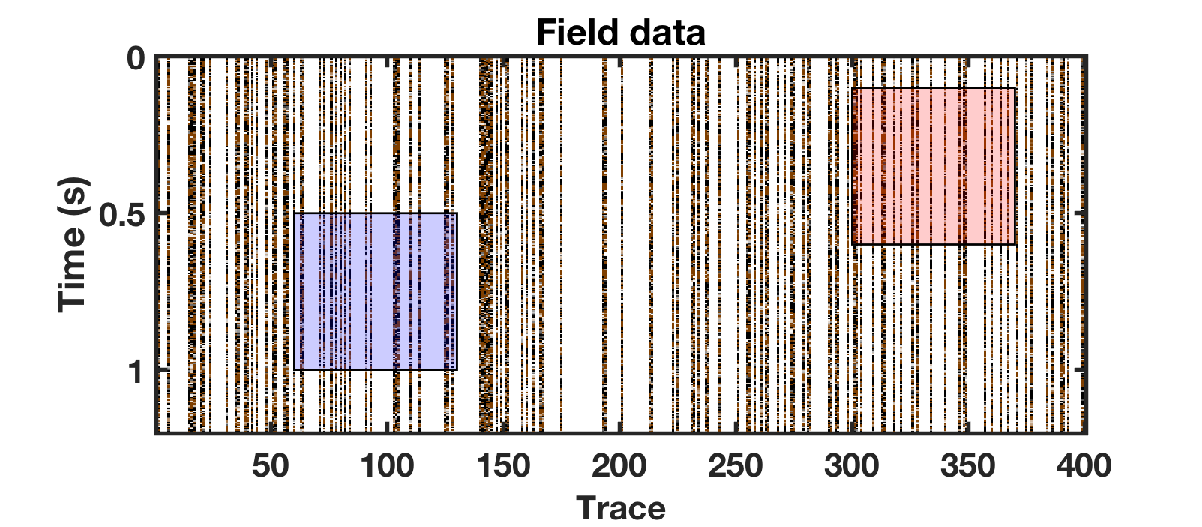
\includegraphics[width=\textwidth]{Fig/field_d0_0}
%	\caption{Real data example \new{with a lot of missing traces}. \new{Because of the difficulty in display a 5D dataset, only one common midpoint gather is extracted and rearranged into a 2D matrix, and is plotted here. The two transparent colored windows denote two zooming areas for an amplified comparison.}}
%	\label{fig:field_d0_0}
%\end{figure}
%
%
%\begin{figure}
%	\centering
%	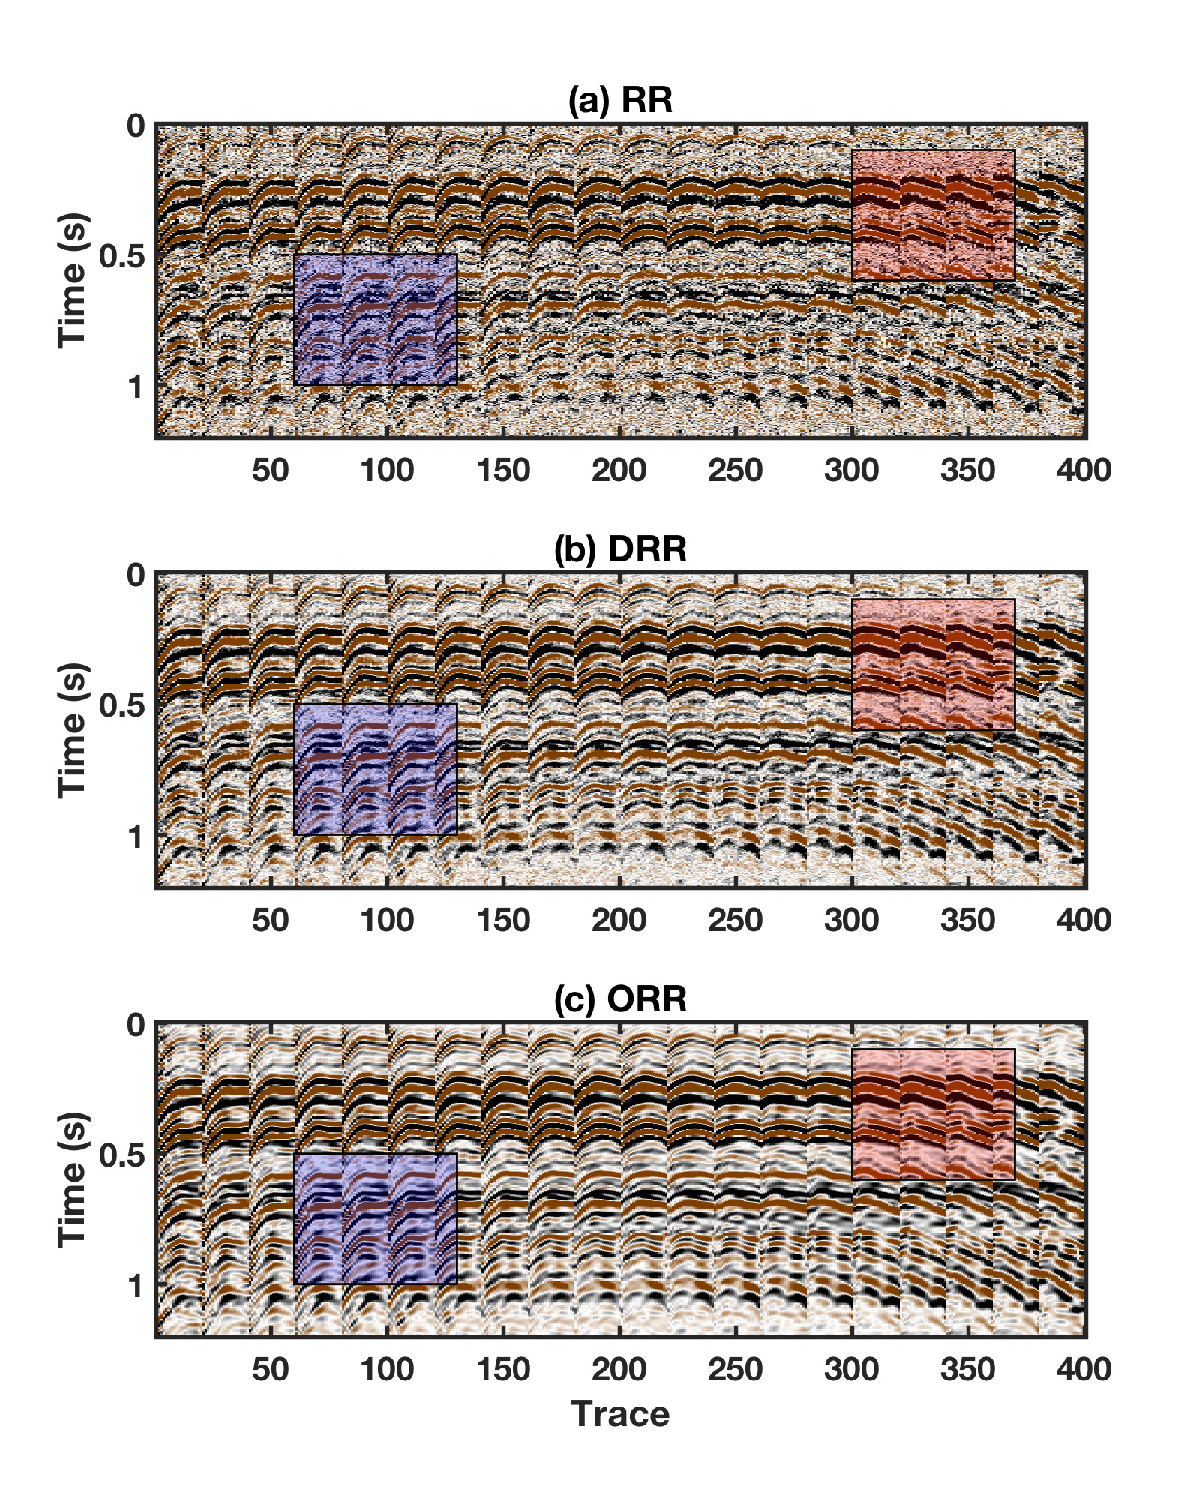
\includegraphics[width=0.9\textwidth]{Fig/field_dn_N12_0}
%	\caption{Real data example. (a) Reconstructed data using the RR method. (b) Reconstructed data using the DRR method. (c) Reconstructed data using the ORR method.  In this case, $rank=20$. \new{It is obvious that all three methods obtain dramatic improvement from the raw data. The ORR method obtains cleaner and spatially more coherent seismic events compared with other two methods.}}
%	\label{fig:field_dn_N12_0}
%\end{figure}
%
%\begin{figure}
%	\centering
%	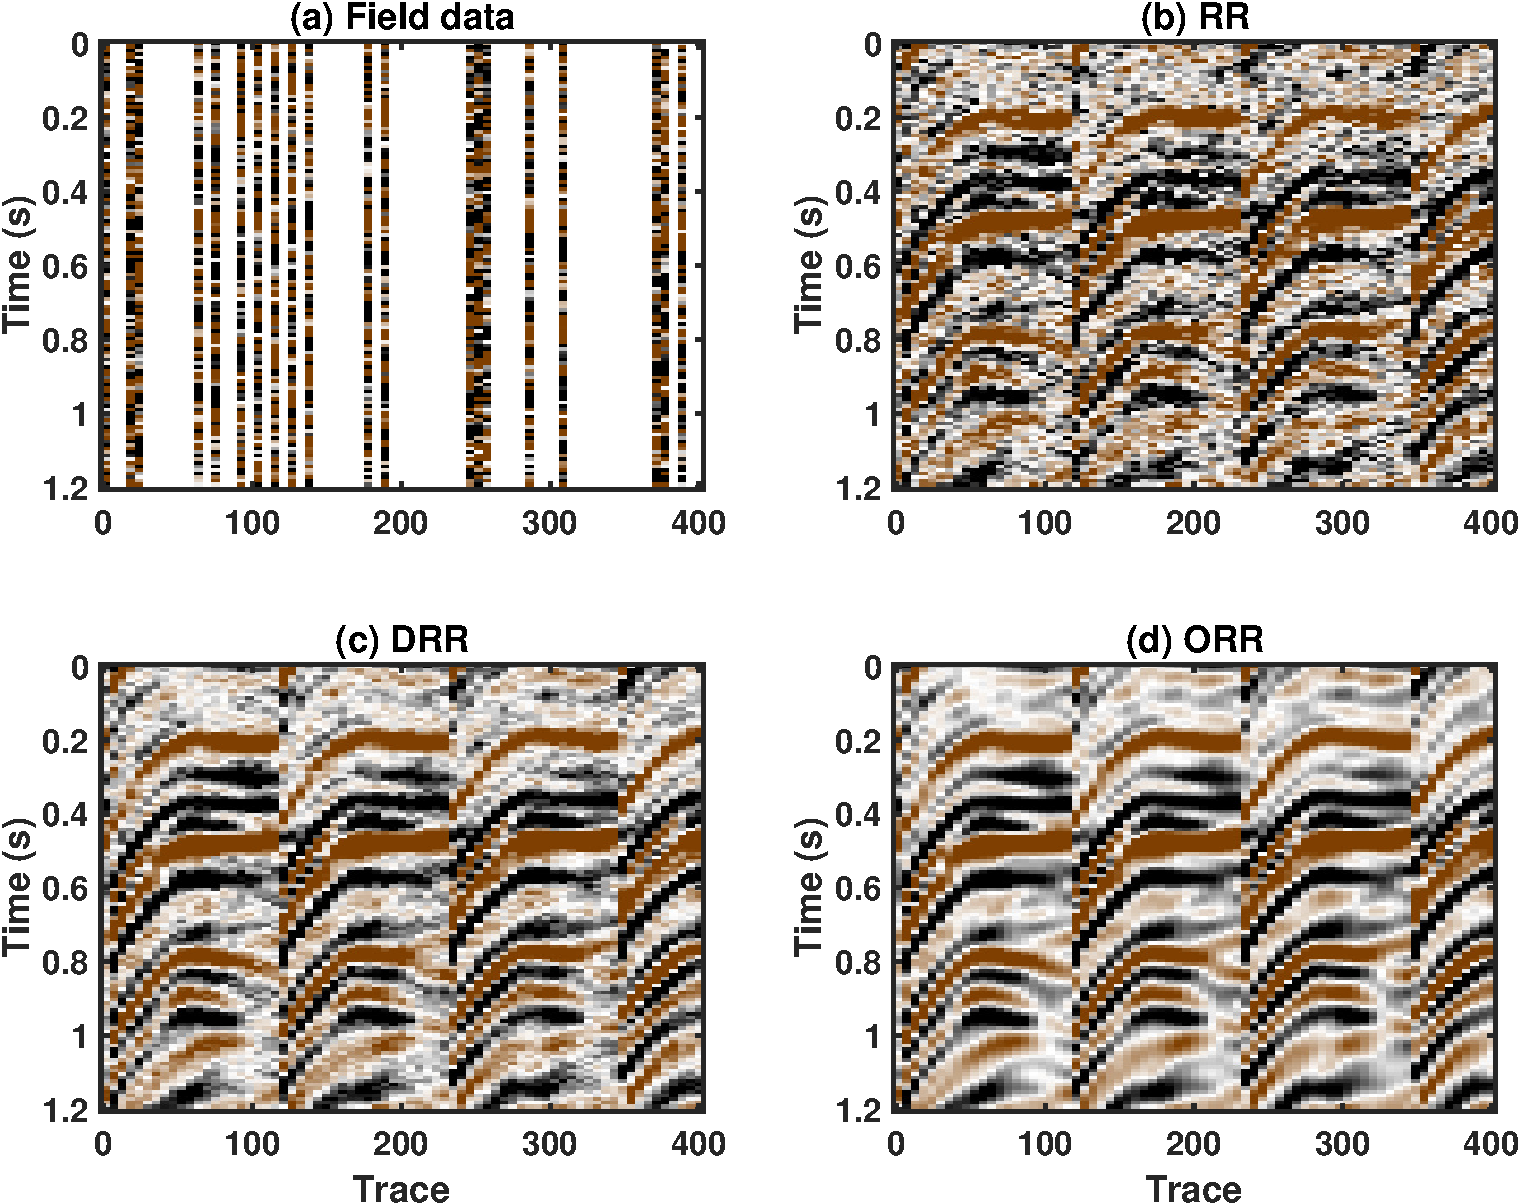
\includegraphics[width=\textwidth]{Fig/field_dn_N12_z1}
%	\caption{Zoomed comparison for the field data example (the blue frame box). (a) Incomplete data. (b) Reconstructed data using the RR method. (c) Reconstructed data using the DRR method. (d) Reconstructed data using the ORR method. }
%	\label{fig:field_dn_N12_z1}
%\end{figure}
%
%\begin{figure}
%	\centering
%	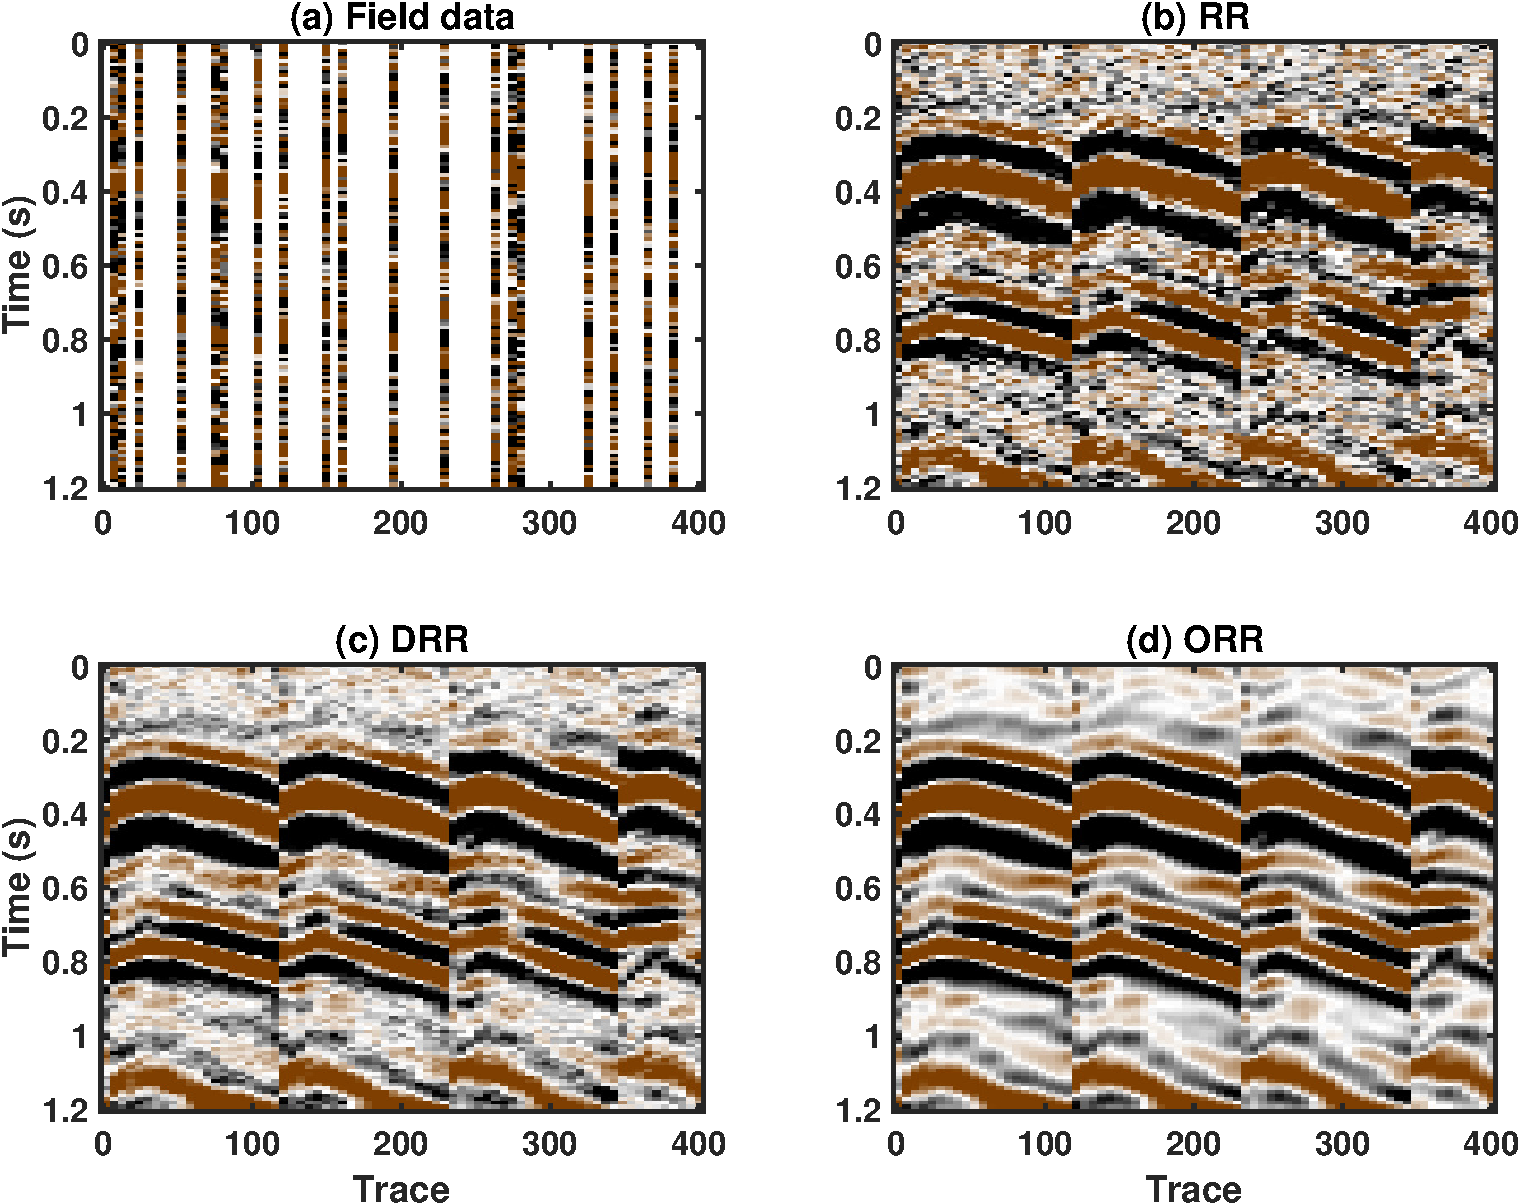
\includegraphics[width=\textwidth]{Fig/field_dn_N12_z2}
%	\caption{Zoomed comparison for the field data example (the red frame box). (a) Incomplete data. (b) Reconstructed data using the RR method. (c) Reconstructed data using the DRR method. (d) Reconstructed data using the ORR method. }
%	\label{fig:field_dn_N12_z2}
%\end{figure}
%
%\begin{figure}
%	\centering
%	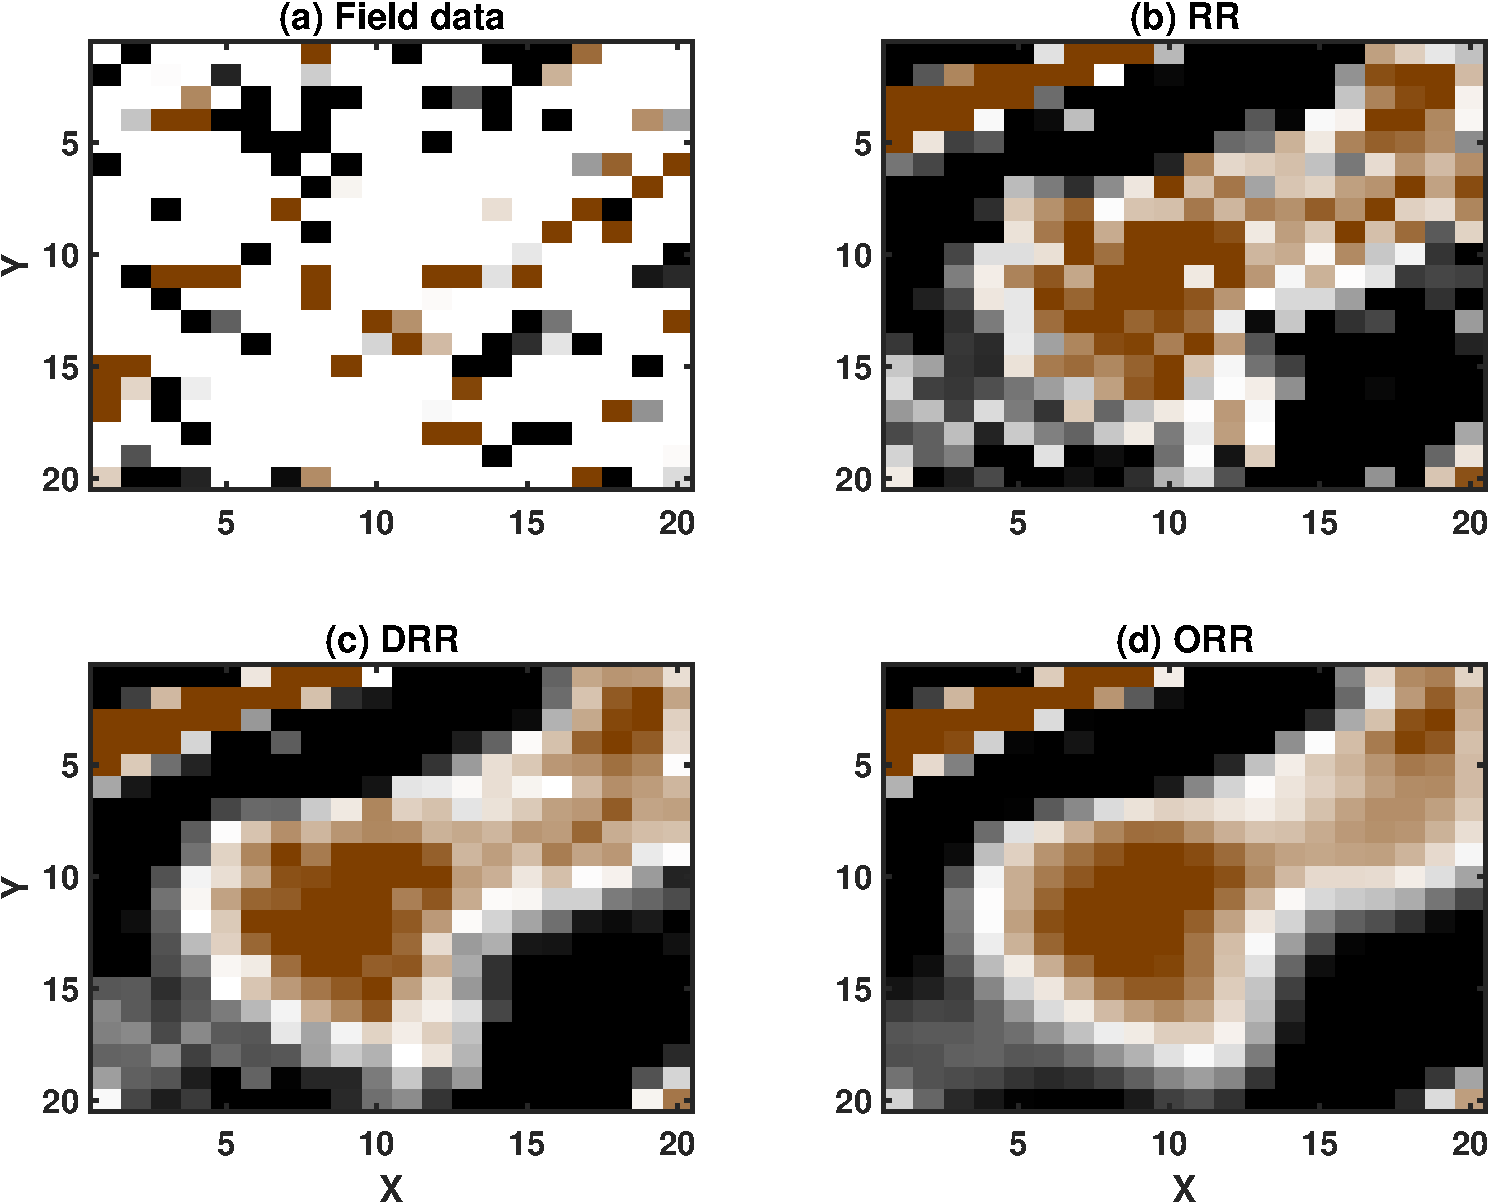
\includegraphics[width=\textwidth]{Fig/field_dn_N12_t80}
%	\caption{Comparison for constant time slice for the field data example ($t=0.32$s). (a) Incomplete data. (b) Reconstructed data using the RR method. (c) Reconstructed data using the DRR method. (d) Reconstructed data using the ORR method. }
%	\label{fig:field_dn_N12_t80}
%\end{figure}
%
%\begin{figure}
%	\centering
%	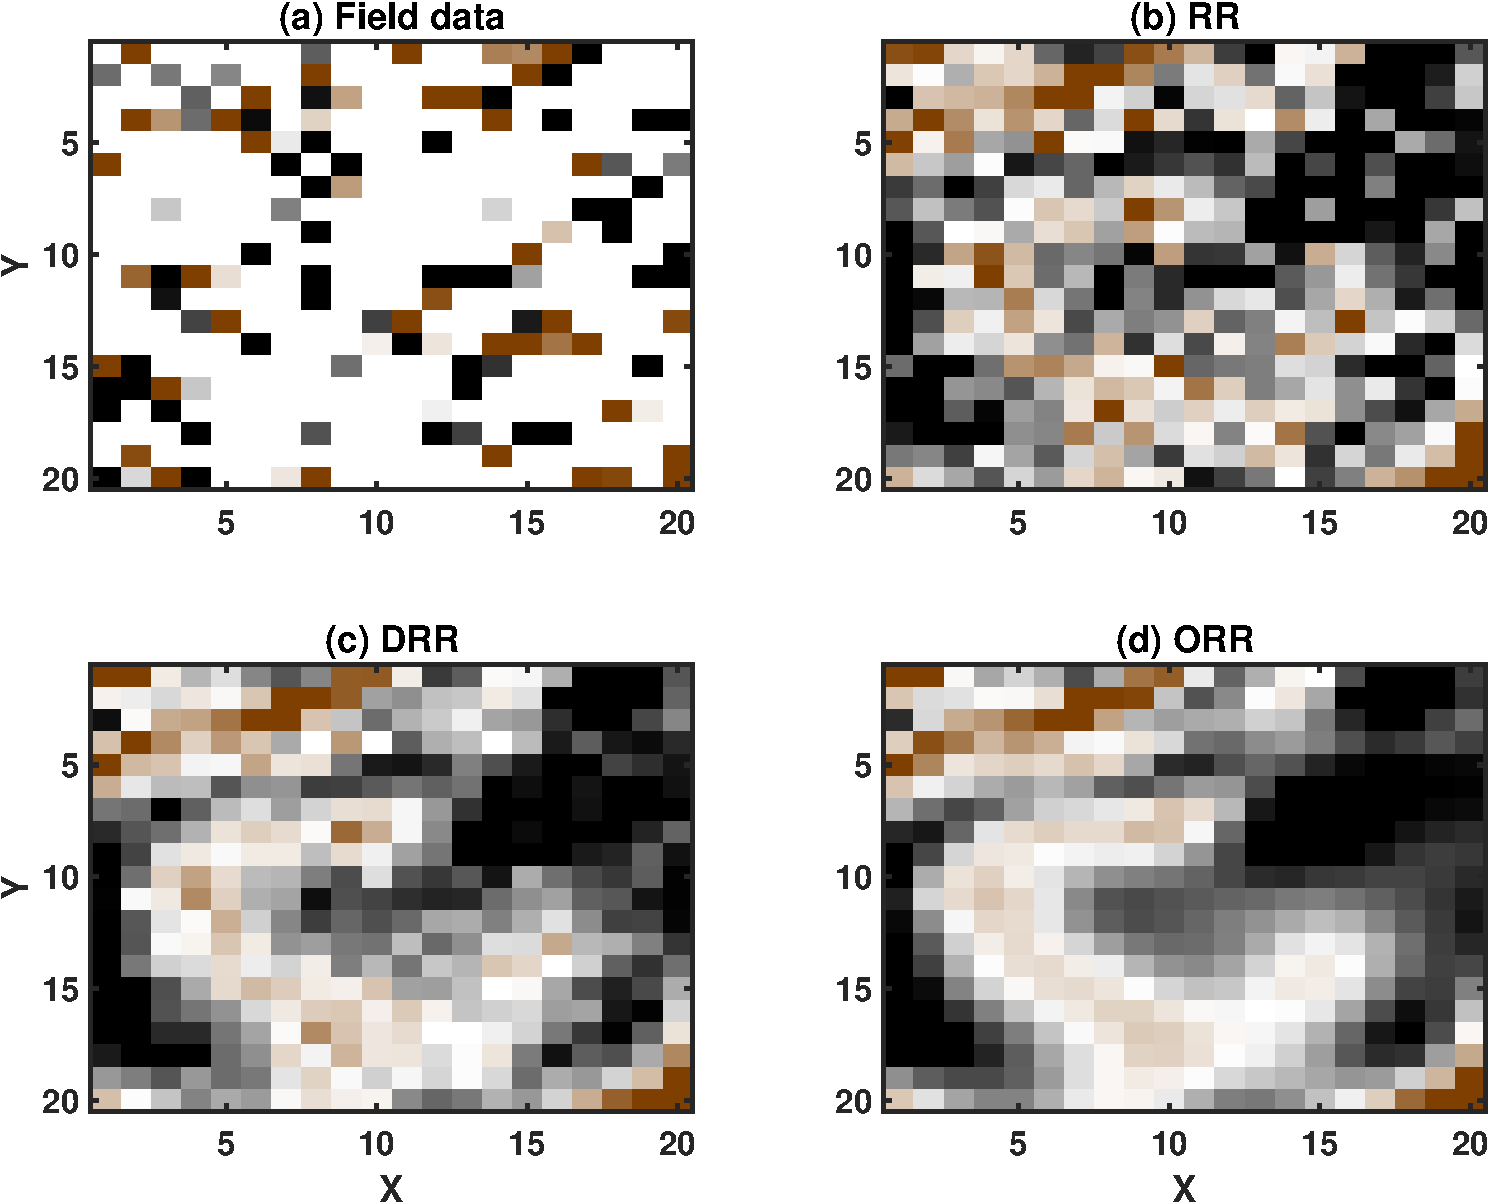
\includegraphics[width=\textwidth]{Fig/field_dn_N12_t160}
%	\caption{Comparison for constant time slice for the field data example ($t=0.64$s). (a) Incomplete data. (b) Reconstructed data using the RR method. (c) Reconstructed data using the DRR method. (d) Reconstructed data using the ORR method. }
%	\label{fig:field_dn_N12_t160}
%\end{figure}

}


To test the sensitivities of each method to input noise level, we vary the variance of the additive random noise from 0.1 to 0.9 and calculate the output SNRs corresponding to different methods and draw the diagrams in Figure \ref{fig:synth_vars}. The black line corresponds to the input SNR curve. The blue, red, and green lines correspond to the RR, DRR, and ORR methods, respectively. As the noise variance increases, the input SNR decreases, and so do the output SNRs of the three methods. However, the proposed method always outperforms the other two methods. It is worth noting that as the noise variance becomes larger, the differences between the proposed method and the other methods are also larger, which indicates that the proposed method is more effective for stronger noise.

To test the effectiveness of each method in situations with different sampling ratios, we vary the sampling ratio from 10\% to 90\%, and draw the input and output SNR curves in Figure \ref{fig:synth_ratios}. The colorful lines have the same meaning in this case. As we can see from Figure \ref{fig:synth_ratios}, the input SNR decreases with increasing sampling ratio. The output SNRs increase with increasing sampling ratios. It is clear that the output SNR curve of the proposed method is always above the other curves. The proposed method outperforms other two methods more when sampling ratio is higher. 

To test the sensitivities of different methods to the input parameter, i.e., the predefined \old{appealing rank}\new{rank}, we vary the rank from 4 to 15 and draw the SNR curves in Figure \ref{fig:synth_ranks}. Both RR and DRR methods decrease fast as the predefined rank increases while the SNR curve of the proposed ORR method is almost flat and is also above the other two curves. This test indicates that while the RR and DRR are more or less sensitive to the predefined rank, the proposed method is almost parameter-free, which makes the ORR method convenient to use in realistic situations. 

To compare the computational cost of different methods, we measure the computing time for the synthetic example with linear events. The computation is done on a MacBook Pro laptop equipped with an Intel Core i7 CPU clocked at 2.5 GHz and 16 GB of RAM. The detailed computing time comparison is shown in Table \ref{tbl:time}. It shows that the computational cost of the ORR method is higher than the other two methods.  The RR and DRR methods have almost the same computational cost while the proposed method costs 2-5 times more than the other two methods. 

In order to test the effectiveness of the three methods on data containing curved events and to compare the performances of different methods in this case, we then use the second example to show the performance.  Figure \ref{fig:hyper_N12} shows the clean data, noisy data, and incomplete data with 70\% traces randonly missing in a common midpoint gather. Figure \ref{fig:hyper_dn_N12} shows the reconstructed data using different methods. Because this dataset no longer meet the linear-event assumption of the rank-reduction based methods, we use a relatively higher rank in this example. The top row in Figure \ref{fig:hyper_dn_N12} shows results when $rank = 12$. The bottom row in Figure \ref{fig:hyper_dn_N12} shows results when $rank = 24$. It is clear that the three methods also work when there are curving events. The proposed method obtains obviously cleaner result than the other two methods. The SNRs of the incomplete data, data from the RR method, DRR method, and ORR method are 0.59, 14.11, 16.46, and 16.86 dB when $rank=12$ and are 0.59, 13.88, 16.01, and 16.83 dB when $rank=24$. We also calculate the local similarity between the exact solution shown in Figure \ref{fig:hyper_d_3v} and each reconstructed data and show the similarity cubes in Figure \ref{fig:hyper_simi_N12}. The local similarity corresponding to the proposed method is obviously higher than those from the  other two methods, indicating a more accurate reconstruction result using the proposed method. 

Finally, we apply the three methods to a 5D field data. We use the data previously used in \cite{yangkang2016irr5d}.  The data have been binned onto a regular grid and a common offset gather of the field data is shown in Figure \ref{fig:field_d0_0}. \new{In Figure \ref{fig:field_d0_0}, the colored stripes are the recorded seismic traces. The white blanks denote the missing traces, which means that we do not observe seismic data in these positions. Because of the difficulty in displaying a 5D dataset, we only show a common midpoint gather here. The 3D common midpoint gather is rearranged into a 2D matrix for a better view. The two transparent colored windows denote two zooming areas for an amplified comparison. } %Although we are only allowed to show a small portion of the field data and to give a limited discussion based on the performance, the comparison between traditional and proposed rank-reduction methods is adequate to show the superior performance of our proposed method. 
In this example, roughly 80\% traces are missing from the regular grids. \new{Because of the high ratio of missing traces, the observed seismic traces do not show any spatial coherency. It is difficult to see the waveforms from the raw data. }
The results from the three aforementioned methods are shown in Figure \ref{fig:field_dn_N12_0}. \new{After 5D reconstruction, the white blanks in the raw data have been filled with seismic traces. The waveforms become well aligned along the spatial direction. Compared with the raw data, all methods seem to obtain a dramatic improvement on the data quality.} It is salient that both DRR and ORR methods obtain \old{very encouraging}\new{much smoother and cleaner} results while the traditional RR method obtain a result that is noisier. \new{Because of the strong residual noise in the result from the traditional RR method, the spatial coherency of the seismic events are deteriorated, which may affect the subsequent processing tasks like imaging, inversion, and interpretation. } When zooming the data in \old{two areas, as highlighted by }the \new{two} transparent blue and red rectangles in both Figures \ref{fig:field_d0_0} and \ref{fig:field_dn_N12_0}, the comparison among different methods becomes much clearer. From Figures \ref{fig:field_dn_N12_z1} and \ref{fig:field_dn_N12_z2}, we observe that although the DRR method obtain a much smoother result compared with the RR result, as already discussed from \cite{yangkang2016irr5d}, the ORR method obtains a even smoother result, with energy spatially more correlative. We also extract two constant time slices at $t=0.32s$ and $t=0.64s$, respectively, and show them in Figures \ref{fig:field_dn_N12_t80} and \ref{fig:field_dn_N12_t160}. The pixels corresponding to the proposed method are obviously smoother from the proposed method. \new{The two reconstructed time slices from the proposed method show obvious shapes of a dome.  }


%\section{Discussions}
\section{Conclusions}
We have introduced a new rank-reduction (RR) method for interpolating and denoising five-dimensional seismic data based on a \new{cascaded }optimal weighting \old{strategy}\new{ and damping operations}. The proposed \new{optimally damped} rank-reduction (ORR) method can further improve \old{our previously developed}\new{the} damped rank-reduction (DRR) method in causing less residual noise and making the result smoother. The proposed ORR method works effectively in various data examples including data with linear/planar events, data with hyperbolic events, and field data. While in the case of low SNR, all rank-reduction methods tend to damage some useful energy, the proposed ORR method does not cause extra damage but can remove more noise than the other rank-reduction methods. The waveforms reconstructed from the proposed method are more similar to the ground-truth solution in the synthetic tests. The block Hankel matrix from the proposed method in each frequency slice is smoother than other rank-reduction method, which accounts for why it is more capable of suppressing residual noise. The proposed method outperforms the other rank-reduction methods more in stronger noise and higher sampling ratios. The effectiveness is almost unchanged for different predefined ranks, meaning that the proposed method is almsot parameter-free. One drawback of the proposed method is that the computational cost is 2-5 times higher than the other rank-reduction methods, which can be potentially tackled in future research.


\section{Acknowledgements}
We would like to thank Dong Zhang and Weilin Huang for inspiring discussions. \new{We also thank Frederik Simons and two anonymous reviewers for constructive suggestions that greatly improved the manuscript.} The research is supported by the starting fund from Zhejiang University and the ``Thousand Youth Talents Plan of China''.


%\subsection{Appendix: local similarity}
% Local similarity between vectors $\mathbf{a}$ and $\mathbf{b}$ is defined as:
%\begin{equation}
%\label{eq:local}
%\mathbf{c}=\sqrt{\mathbf{c}_1\circ\mathbf{c}_2}
%\end{equation}
%where $\circ$ denotes dot product, $\mathbf{c}_1$ and $\mathbf{c}_2$ come from two least-squares minimization problems:
%\begin{align}
%\label{eq:local1}
%\mathbf{c}_1 &=\arg\min_{\mathbf{c}_1}\Arrowvert \mathbf{a}-\mathbf{B} \mathbf{c}_1 \Arrowvert_2^2 \\
%\label{eq:local2}
%\mathbf{c}_2 &=\arg\min_{\mathbf{c}_2}\Arrowvert \mathbf{b}-\mathbf{A} \mathbf{c}_2 \Arrowvert_2^2
%\end{align}
%where $\mathbf{A}$ is a diagonal operator composed of the elements of $\mathbf{a}$, $\mathbf{B}$ is a diagonal operator composed of the elements of $\mathbf{b}$. Note that in equations \ref{eq:local}-\ref{eq:local2}, $\mathbf{a}$, $\mathbf{b}$, and $\mathbf{c}$  denote vectorized 2D matrices. Equations \ref{eq:local1} and \ref{eq:local2} can be solved using shaping regularization with a local-smoothness constraint:
%\begin{align}
%\label{eq:local3}
%\mathbf{c}_1 &= [\lambda_1^2\mathbf{I} + \mathbf{T}(\mathbf{B}^T\mathbf{B}-\lambda_1^2\mathbf{I})]^{-1}\mathbf{TB}^T\mathbf{b},\\
%\label{eq:local4}
%\mathbf{c}_2 &= [\lambda_2^2\mathbf{I} + \mathbf{T}(\mathbf{A}^T\mathbf{A}-\lambda_2^2\mathbf{I})]^{-1}\mathbf{TA}^T\mathbf{a},
%\end{align}
%where $\mathbf{T}$ is a smoothing operator and $\lambda_1$ and $\lambda_2$ are two parameters controlling the physical dimensionality and enabling fast convergence when inversion is implemented iteratively. These two parameters can be chosen as $\lambda_1  = \Arrowvert\mathbf{B}^T\mathbf{B}\Arrowvert_2$ and $\lambda_2  = \Arrowvert\mathbf{A}^T\mathbf{A}\Arrowvert_2$.
%
\bibliographystyle{seg}
\bibliography{dos5d}


\newpage
\listoftables

\newpage
\listoffigures
\newpage


\begin{table}[h]
\caption{SNRs comparison in dB for the synthetic example with linear events.}
\begin{center}
     \begin{tabular}{|c|c|c|c|c|} 
	  \hline &Incomplete & RR  & DRR  & ORR \\ 
	  \hline N=3    & -4.59 & 9.96 & 11.68 & 12.03 \\	  
	  \hline N=5    & -4.59 & 8.01 & 10.87 & 11.99 \\
	  \hline N=10 & -4.59 & 5.51 & 9.54 & 11.83 \\
%	  \hline N=15 &  &  &  &  \\
       \hline
    \end{tabular} 
\end{center}
\label{tbl:plane}
\end{table}

\begin{table}[h]
\caption{Computing time comparison in seconds for the synthetic example with linear events. The computation is done on a MacBook Pro laptop equipped with an Intel Core i7 CPU clocked at 2.5 GHz and 16 GB of RAM.}
\begin{center}
     \begin{tabular}{|c|c|c|c|c|} 
	  \hline  & RR  & DRR  & ORR \\ 
	  \hline N=3    &246.39  & 249.63 & 656.33   \\	  
	  \hline N=5    &249.37  & 252.52 &    923.45\\
	  \hline N=10  &250.28  &  255.27 & 1226.63 \\
%	  \hline N=15 &  &  &  &  \\
       \hline
    \end{tabular} 
\end{center}
\label{tbl:time}
\end{table}

\begin{table}[h]
\caption{SNRs comparison in dB for the synthetic example with hyperbolic events.}
\begin{center}
     \begin{tabular}{|c|c|c|c|c|} 
	  \hline &Incomplete  & RR  & DRR & ORR \\ 
	  \hline N=12& 0.59 & 14.11 & 16.46 & 16.86 \\
	  \hline N=24& 0.59 & 13.88 & 16.01 & 16.83 \\
       \hline
    \end{tabular} 
\end{center}
\label{tbl:hyper}
\end{table}
\newpage
%\inputdir{test}
%\plot{test1}{width=\textwidth}{Separated x-component of the S1 elastic wavefield in the orthorhombic media.}
%\multiplot{2}{test1,test2}{width=0.45\textwidth}{(a) Caption a. (b) Caption b.}







%In equation \ref{eq:M_a}, because $\mathbf{U}_1^M$ and $\mathbf{V}_1^M$ both have orthonormal columns (as they come from the SVD of $\mathbf{M}$), thus equation \ref{eq:M_a} is an SVD of $\hat{\mathbf{M}}$. Let 
%\begin{equation}
%\label{eq:Sigma_new}
%\hat{\boldsymbol{\Sigma}}_1^M=\hat{\mathbf{W}}\boldsymbol{\Sigma}_1^M,
%\end{equation}
%and thus $\hat{\boldsymbol{\Sigma}}_1^M$ denotes the new singular values of the the estimated signal component after weighting. 


%\AtEndDocument{}


%\begin{figure}
%	\centering
%	\subfloat[]{\includegraphics[width=0.8\textwidth]{Fig/fig}}
%	\caption{Caption.}
%	\label{fig:fig}
%\end{figure}


%\begin{figure}
%	\centering
%	\subfloat[]{\includegraphics[width=0.45\textwidth]{Fig/fig1}
%    \label{fig:fig1}}\\
%    \subfloat[]{\includegraphics[width=0.45\textwidth]{Fig/fig2}
%    \label{fig:fig2}}\\
%	\caption{(a) Caption a. (b) Caption b.}
%	\label{fig:fig1,fig2}
%\end{figure}

%\begin{table}[h]
%\caption{Table caption}
%\begin{center}
%     \begin{tabular}{|c|c|c|c|c|c|} 
%	  \hline Column1 (unit)  & Column2 (unit) & Column3 (unit) \\ 
%	  \hline 1 & 2  & 3 \\
%       \hline
%    \end{tabular} 
%\end{center}
%\label{tbl:table1}
%\end{table}

